\chapter{Context-Dependent Environments: \\ A Parameterization Paradigm for Hardware Generators}
\label{c.parameters}

As Moore's law fails, increasing demand for computational efficiency is no longer being matched by gains from process scaling. 
Instead, chip designers are improving efficiency by combining special-purpose accelerators with general-purpose processors in increasingly heterogenous systems-on-chip.
In this new world of energy-efficient, heterogeneous, application-specific designs, it will be essential to both improve the productivity of hardware designers as well as enable extensive design-space exploration \cite{shacham-micro10}.

Since it is not possible to build custom chips from scratch for every application,
we need hardware design tools that allow us to capture decisions made
during the process of designing one chip and easily make them differently when tackling a new target.
Creating parameterized hardware generators rather than individual design instances not only allows for application-specific customization of the final hardware,
but also gives designers the capability to preserve
knowledge related to performance and energy trade-offs from previous design iterations.
By parameterizing aspects of the design, we can scale it from test chip sizes to final product without rewriting any modules, amortizing verification costs and increasing the validation confidence over time without rewriting code.
This approach is integral to our agile aproach to hardware design.

The most salient feature of a hardware generator or template compared to a single design instance is that certain features of the design are left under the control of the user deploying it within their chip.
We term these features the {\em parameters} of the generator.
Parameterization is the process by which a generator instantiates a particular design by supplying values for each parameter.
By searching over the top-level parameters exposed by a set of such generators, chip designers can explore tradeoffs between performance, area, and energy efficiency.
By recording the outcomes of these explorations, designers can build up a map of how to customize their design for a particular application domain.

From the perspective of the author of a hardware generator, it is impossible to know the full instantiation context of their component, so the goal is to expose as many parameters as possible while also recording any constraints the internals of the design put on those parameters' values.
The parameters and their constraints become the interface through which the generator author and the system architect communicate, and define boundaries of the space of designs which it is possible to explore.

Parameterization is clearly a first-order concern in the creation of tools based around custom hardware generation.
In order to use generators productively, we need to understand how the choice of parameterization paradigm affects designers.
We claim that the mechanism by which hardware generators are parameterized can greatly influence three metrics of design robustness: reusability, composability, and modularity.
We define these three metrics as follows:
\begin{description}
\item[Resuing] modules means that they can be instantiated in different hardware contexts with no internal source code changes, only differing parameterizations. Reusability amortizes verification overhead.
\item[Composing] modules requires all parameter constraints and dependencies to be explicit and exposed to the user. Composability is mandatory to build up large designs consisting of multiple generators.
\item[Modifying] a generator by changing its parameters should not cause a cascade of changes throughout any nested modules which instantiate that generator's output. Modularity avoids accruing technical debt in the face of changing generator capabilities.
\end{description}

This chapter first provides a taxonomy of existing parameterization paradigms in hardware description languages,
and evaluates them in terms of the above metrics.
We then introduce a new parameterization paradigm, called \emph{context-dependent environments} (CDEs).
In the CDE paradigm, a key-value environment is passed down a hardware module hierarchy, and the value returned for each query can depend on other parameter values at that query's origin within the design.
The encapsulation of many parameters into a single object coupled with context-specific lookups preserves module reusability and composition, while also improving a generator's robustness to any external module hierarchy modifications.

We provide both a case study and a formal analysis of design robustness with respect to each of the paradigms and prove that CDEs are the most robust option.
We then provide examples of how our open-source Scala implementation of CDEs is used in various sub-components of our RocketChip generator.
As we will see, even a design choice as complicated and pervasive as a multi-level cache coherence protocol can be made a tuneable design parameter when properly factored out from the rest of the design. 
By providing support for generating a family of protocols rather than one single protocol, my thesis has enabled us to iterate on protocol design as we scale up the size of the memory hierarchy across chip iterations.

\section{Background}
\label{sec:rel}

Unlike high-level synthesis tools that transform abstract descriptions of a computation into gates, hardware generators are parameterized, programmatic descriptions of how to elaborate a templated RTL module hierarchy\cite{templates}.
Given a set of top-level configurations that supply value bindings for individual parameters, a generator can construct a vast number of different designs from a single piece of templated source code.
Hardware generators are an increasingly popular paradigm; examples include Stanford's FPU generator\cite{fpu}, Lawrence Berkeley National Lab's OpenSoC\cite{opensoc}, and UC Berkeley's Rocket Chip Generator\cite{rocket}.
Bluespec provides AzureIP Libraries\cite{azure} to give designers reusable components for use in custom generators. 
Support for parameterization is a critical feature of the language in which the generator is written.

Unfortunately, many traditional hardware description languages lack the language features to support parameterization paradigms that make hardware generator composition tractable for large, heterogenous designs.
Section \ref{sec:tax} discusses how existing parameterization paradigms in Verilog, VHDL, SystemVerilog and Bluespec SystemVerilog limit design modifiability, manifesting in cascades of source code changes when inserting new parameters into modules or when making changes to the module hierarchy.
In contrast, embedded HDLs, such as Genesis2\cite{genesis2} and Chisel\cite{chisel}, can leverage features of their host programming language to give the designer flexibility and power when describing the parameterization of their design.
Moving beyond built-in host language features, we are also free to construct our own parameterization frameworks written in the host language, and intermingle use of these frameworks with the hardware generation capabilities of our embedded HDL.

%Genesis 2: Hardware elaboration language that hosts hardware generators (architectural parameterization -> hardware specification). Leverages SystemVerilog to describe actual hardware description. Builds module tree where each module has a parameter environment. Each can use relative and absolute module paths for inter-module parameter references. Outputs XML to encapsulate full ``configuration'', meaning the text description of how SystemVerilog module declarations are composed. Would need to explicitly rename parameters, can do this in multiple ways, including defining synonyms or referencing a parent's parameter. Adding parameters does require explicit renaming, no mechanism to reference child. Adding cde's would only benefit it, I think.

This opportunity inspired us to examine parameterization solutions that have been investigated in software contexts.
Lisp languages explored tradeoffs between dynamic scoping and lexical scoping \cite{gordon}.
With lexical scoping, in order to bind a name to an entity we first search in the local function, then the scope in which this function was defined, and so on.
``Lexical'' in this case refers to the text of the source code itself.
Lexical scoping provides referential transparency, which is a boon for both the programmer and compiler.
With dynamic scoping, we again search first in the local function, but then search the function that called this function, and so on up the call stack of the running program.
``Dynamic'' in this case refers to the fact that the call stack can be different every time a given function is called, and so the binding created for the variable can thereby differ as well.
Dynamic binding is useful as a substitute for globally scoped variables, and is excellent for deep customization of nested subsystems.

While lexical binding is now the norm for most programming languages, many mechanisms have been developed to allow programmers to explicitly tie in dynamic binding benefits where they are useful.
These include special binding forms in most Lisp's (\code{fluid-let} in Scheme \cite{steele} and \code{parameterize} in Racket \cite{flatt2013racket}), implicit parameters \cite{lewis2000implicit}, and the Reader monad of Haskell \cite{jones1995functional}.
While these approaches all focus on re-enabling the parameterization flexibility of dynamic binding in a more controlled manner, 
the context-dependent environments we propose here are actually a strictly more powerful mechanism than dynamic binding. 

\section{Taxonomy of Extant Hardware Parameterization Paradigms}
\label{sec:tax}

Before introducing context-dependent environments, we first define and examine three existing parameter-passing paradigms: argument lists, structs, and dynamic environments.
We examine how these paradigms are used in hardware description languages and evaluate them in terms of a simple case study.

\begin{description}
\item[Argument Lists.] The default, lexical binding approach wherein all parameters are explicitly passed to the constructor of each hardware module.
\item[Structs.] A more sophisticated lexcical binding approach wherein user-defined datatypes are used to abstract away the specific parameters
\item[Environments.] A dynamic binding approach wherein a key-value store
\end{description}

Each of these approaches attempts to maximize design modularity and reusability by first binding all parameter names at the top level of the module hierarchy and then requesting necessary parameter values within each module. 
While default values could be supplied locally, any parameters used in inter-generator design space exploration must be exposed at the top level of each generator.

%TODOEach scheme preserves module modularity and reusability by expressing all parameters at the top level and only requesting necessary parameters. We evaluate each paradigm's robustness by adding parameters/modules and counting the number of top-level (TLCs), non-local (NLCs), or local (LCs) source code changes cascading from this initial modification.

%TODOTLCs are updates to parameter assignments at module hierarchy's root. An LC is the original insertion/deletion/modification of a module instantiation, while NLCs are all additional changes passing the TLCs parameter value to the LCs module instantiation. The ideal parameterization paradigm eliminates all NLCs and limits the number of LCs and TLCs.

%TODOThe following sections use examples written in Verilog-like pseudo-code which ignores non-parameter related statements/expressions. Below is the syntax for struct declaration, module declaration, and other object instantiations:
We can evaluate the robustness of these parameterization paradigms by adding new parameters or modules and examining the source code changes that are required as a result of this initial modification to the design.
We differentiate three types of source code changes.
Local changes (LCs) are the initial insertion or modification of a module instantiation. 
Top-level changes (TLCs) are new parameter assignments made at the top  of the module hierarchy. 
Non-local changes (NLCs) are all the additional changes required to pass a top-level parameter value (created by a TLC) to a lower-level module instantiation (created by an LC). 
The ideal parameterization paradigm eliminates all NLCs and limits the number of LCs and TLCs for a given design modification.

The following sections use examples written in Verilog-like pseudo-code which elides non-parameter-related expressions. Here is the syntax for object declaration and instantiation:

\begin{phdl}
struct S {f:Bool,g:Int}          // struct declaration
module A #(p1,p2,p3,p4,p5)(...): ... 
   // module declaration: parameters use 1st argument list #(p1,...)
   // other RTL constructs like IOs use 2nd argument list (not shown)
module B ()(...):
  a = new S(true, 1)             // struct instantiation
  b = a.f                        // struct access
  A #(a,b,c,d,e) myA (...)       // module instantiation
\end{phdl} 

\subsection{Argument List Parameterization}

\emph{Argument list parameterization} is when parameters are passed-by-value through modules' constructor function arguments. 
Verilog and VHDL are examples of existing HDLs that solely support this paradigm. 

The following example illustrates how this paradigm is brittle to modifications. All top-level parameters are declared then passed directly via \code{Tile's} argument list. These values are propagated down the module hierarchy via the \code{Core} and \code{Cache} argument lists:

\begin{phdl}
module Top#()():
  fpu? = true    // Whether our core should instantiate an FPU
  icSize = 256   // Size of the instruction cache
  dcSize = 512   // Size of the data cache
  Tile #(fpu?,icSize,dcSize) myTile (...)
module Tile #(fpu?,icSize,dcSize)(...):
  Core  #(fpu?) myCore (...)
  Cache #(icSize) myIcache (...)
  Cache #(dcSize) myDcache (...)
  assert (icSize < dcSize) ...
module Cache #(size)(...):... // icSize/dcSize implicitly renamed size
module Core #(fpu?)(...) :
  Queue myIQ (...) ...
\end{phdl} 

If we modify \code{Core} to use a parameterized queue, \code{PQueue \#(size)}, we must make: (1) a LC for \code{PQueue's} instantiation within Core; (2) a TLC for \code{Top's} parameter declaration list; (3) four NLCs for \code{Tile} and \code{Core}'s declaration parameter list, and \code{Tile} and \code{Core}'s instantiation:

\begin{phdl}
module Top #()():
  (*@\textcolor[rgb]{1,0,0}{iqSize = 32}@*)  // Size of issue queue                            // TLC
  fpu? = true
  icSize = 256 
  dcSize = 512
  Tile #(fpu?,icSize,dcSize,(*@\textcolor[rgb]{1,0,0}{iqSize}@*)) myTile (...)                 // NLC
module Tile #(fpu?,icSize,dcSize,(*@\textcolor[rgb]{1,0,0}{iqSize}@*))(...):                   // NLC
  Core #(fpu?,(*@\textcolor[rgb]{1,0,0}{iqSize}@*)) myCore (...)                               // NLC
  Cache #(icSize) myIcache (...)
  Cache #(dcSize) myDcache (...)
  assert (icSize < dcSize)
module Cache #(size)(...) : ... 
module Core #(fpu?,(*@\textcolor[rgb]{1,0,0}{iqSize}@*))(...) :                                // NLC
  (*@\textcolor[rgb]{1,0,0}{PQueue \#(iqSize) myIQ (...)}@*)  // Add parameterized queue        // LC
module PQueue #(size)(...):... // iqSize implicitly renamed size
\end{phdl}

In summary, adding a parameter to a module triggers many non-local changes. For small designs, the total number of changes might be small. However, as we will see in Section~\ref{sec:scca}, the number of NLCs scales with module hierarchy size, making modifications burdensome under this paradigm.

\subsection{Struct Parameterizations}

SystemVerilog and Bluespec provide user-defined struct types, and these can be used to encapsulate multiple parameters within individual statically-typed objects. These structs can be organized in two ways.

\subsubsection{Flat-Struct Parameterization}

In \emph{flat-struct parameterization}, each module has a unique specialized struct type containing all parameters used by that module and all of its child modules. This scheme eliminates some non-local changes because module constructor argument lists do not grow with additional parameters:

\begin{phdl}
struct tilePars {fpu?:Bool,icSize:Int,dcSize:Int}
struct corePars {fpu?:Bool}
module Top #()():
  fpu? = true    // Whether the core should instantiate an FPU
  icSize = 256   // Size of the instruction cache
  dcSize = 512   // Size of the data cache
  tp = new tilePars(fpu?,icSize,dcSize)
  Tile #(tp) myTile (...)
module Tile #(params)(...):
  cp = new corePars(params.fpu?)
  Core  #(cp) myCore (...)
  Cache #(params.icSize) myIcache (...)
  Cache #(params.dcSize) myDcache (...)
  assert (params.icSize < params.dcSize) ...
module Cache #(size)(...) : ...
module Core #(params)(...) :
  Queue myIQ (...) ...
\end{phdl} 

However, when inserting a \code{PQueue}, this scheme still requires some non-local changes because every parent's parameter struct declaration and instantiation must be changed:

\begin{phdl}
struct tilePars {fpu?:Bool,icSize:Int,dcSize:Int,(*@\textcolor[rgb]{1,0,0}{iqSize:Int}@*)}     // NLC
struct corePars {fpu?:Bool,(*@\textcolor[rgb]{1,0,0}{iqSize:Int}@*)}                           // NLC
module Top #()():
  (*@\textcolor[rgb]{1,0,0}{iqSize = 32}@*)  // Size of issue queue                            // TLC
  fpu? = true
  icSize = 256
  dcSize = 512
  tp = new tilePars(true,256,512,(*@\textcolor[rgb]{1,0,0}{32}@*))                             // NLC
  Tile #(tp) myTile (...)
module Tile #(params)(...):
  cp = new corePars(params.fpu?,(*@\textcolor[rgb]{1,0,0}{params.iqSize}@*))                   // NLC
  Core  #(cp)  myCore   (...)
  Cache #(params.icSize) myIcache (...)
  Cache #(params.dcSize) myDcache (...)
  assert (params.icSize < params.dcSize) ...
module Cache #(size)(...) : ...
module Core #(params)(...) :
    (*@\textcolor[rgb]{1,0,0}{PQueue \#(params.iqSize) myIQ (...)}@*)// Add parameterized queue // LC
module PQueue #(size)(...) : ...]
\end{phdl} 

Putting all top-level parameters into a single flat-struct which is passed to every module in the design
eliminates NLCs but means that sub-modules within the design cannot be reused in other contexts.

\subsubsection{Nested-Structs Parameterization}

To avoid cascading changes to all parent's parameter struct declaration and instantiation, one can use \emph{nested-struct parameterization}. Instead of a module's struct consisting of a flat list of parameters, it contains its parameters as well as the parameter structs for its immediate children. If applied to the previous example, only \code{PQueue's} immediate parent's struct, \code{corePars}, would need modification:

\begin{phdl}
struct corePars {fpu?:Boolean,(*@\textcolor[rgb]{1,0,0}{iqSize:Int}@*)}                        // NLC
struct tilePars {cp:corePars,icSize:Int,dcSize:Int}
module Top #()():
  (*@\textcolor[rgb]{1,0,0}{iqSize = 32}@*)                                                    // TLC
  fpu? = true
  icSize = 256
  dcSize = 512
  cp = new corePars(fpu?,(*@\textcolor[rgb]{1,0,0}{iqSize}@*))                                 // NLC
  tilePars tp (cp,icSize,dcSize)
  Tile #(tp) myTile (...)
module Tile #(params)(...):
  Core  #(params.cp)  myCore   (...)
  Cache #(params.icSize) myIcache (...)
  Cache #(params.dcSize) myDcache (...)
  assert (params.icSize < params.dcSize) ...
module Cache #(size)(...) : ...
module Core #(params)(...) :
    (*@\textcolor[rgb]{1,0,0}{PQueue \#(params.iqSize) myIQ (...)}@*)// Add parameterized queue // LC
module PQueue #(size)(...) : ...
\end{phdl} 

Although the nested-structs approach eliminates almost all NLCs, it presents its own set of problems. 
Suppose we want to add a prefetcher to our instruction cache. 
We append module \code{Prefetch} with a single parameter (\code{distance}) and insert module \code{CacheWithPF} that instantiates our \code{Cache} and \code{Prefetch} modules. 
Unfortunately, this breaks our previously-existing assert statement because the nested structure of the parameter objects explicitly encodes the module hierarchy:

\begin{phdl}
struct corePars {fpu?:Bool,iqSize:Int}
struct tilePars {cp:corePars,icSize:Int,dcSize:Int}
module Top #()():
  iqSize = 32
  (*@\textcolor[rgb]{1,0,0}{dist = 16}@*)    // Distance prefetched                            // TLC
  fpu? = true
  icSize = 256
  dcSize = 512
  (*@\textcolor[rgb]{1,0,0}{cpf = new cachePfPars(dist,icSize)}@*) // Insert cache+prefetcher  // NLC
  cp = new corePars(fpu?,iqSize)
  tp = new tilePars(cp,cpf,dcSize)
  Tile #(tp) myTile (...)
module Tile #(params)(...):
  Core  #(params.cp)  myCore   (...)
  (*@\textcolor[rgb]{1,0,0}{CacheWithPF \#(params.cpf) myIcache (...)}@*)                       // LC
  Cache #(params.dcSize) myDcache (...)
  assert ((*@\textcolor[rgb]{1,0,0}{params.cpf.size}@*) < params.dcSize)                       // NLC
module CacheWithPF #(params)(...)
struct cachePfPars {dist, size}
module Prefetch #(dist)(...) : ...
... // Cache, Core, PQueue module declarations are unchanged
\end{phdl} 

\subsubsection{Summary}

While both struct paradigms are acceptable for small and flat designs, generators often have deep module hierarchies or interoperate with modules from multiple libraries. 
These paradigms embrittle these designs because changes to the module structure break any inter-module parameter reference. 
Note that these broken references can be located anywhere in the design, often not located near the LC; nested-structs cannot guarantee a robust design despite reducing NLCs.

\subsection{Environment Parameterization}
%\subsubsection{Definition and Existing Support}
An \emph{environment} is an immutable key-value store that can be inherited and passed with modifications. While similar to POSIX environments where shell languages have a first-class syntax for accessing environment values (e.g. \$foo), any implementation in an HDL will have to explicitly pass the environment object to query it.

We do not consider similar dynamic scoping solutions such as global constants, preprocessor macros, or global key-value stores because such schemes lack modularity.
They generally do not give the designer a mechanism manage namespace collisions between different third-party generators, 
and, more importantly, they do not allow designers to override values in a context-dependent way when instantiating modules in a heterogenous system.

Unfortunately, SystemVerilog and Bluespec (as well as Verilog and VHDL) cannot support environments as they require either nested functions or HashMaps. %TODO
 While the SystemVerilog language includes associative arrays (similar to HashMaps), most SystemVerilog compilers do not support this language construct. 

Chisel and Genesis2 leverage Scala and Perl, respectively, for module hierarchy elaboration. Because Scala and Perl support first-class functions and maps, both HDLs can support regular environment passing.

% Bluespec requires all type checking be resolved prior to elaboration; since the compiler cannot guarantee that the returned value is type safe, associative arrays are not supported. 

%\subsubsection{Robustness Example}

Our pseudo-HDL can support environments with the following syntax for instantiation, modification, and querying:

\begin{phdl}
x = {'key1' -> 1,'key2' -> 3} // CDE instantiation
y = x ++ {'key1' -> 2}        // CDE modification
print x('key1')               // CDE query, prints '1'
print y('key1')               // CDE query, prints '2'
print y('key2')               // CDE query, prints '3'
\end{phdl}

An important note is that the \code{++}  operator returns a new environment and does not affect the original environment. In addition, all values in key-value pairs are lazily evaluated only when a query matches a key.

In the following example, all modules with two or more parameters now accept an environment parameter:


%This environment could be implemented in Bluespec or SystemVerilog using tagged unions or associative arrays. Unfortunately, both languages do not support dynamically typed parameters and thus cannot pass associative arrays as parameter objects. Tagged unions, however, can be statically-type safe and used if the types of all parameters are known. While both Bluespec and SystemVerilog claim support for tagged unions, many SystemVerilog compilers lack support for them.

%To parameterize a child module, a parent copies its own environment and adds/overwrites any key-value mapping before passing it to the child's parameter list. The original example is shown below using environment passing:

\begin{phdl}
module Top #()():
  topPars = {'fpu?'   -> true, // TLC are only to this environment 
             'icSize' -> 256,
             'dcSize' -> 512}
  Tile #(topPars) myTile (...)
module Tile #(params)(...):
  Core  #(params) myCore (...)
  Cache #(params('icSize')) myIcache (...)
  Cache #(params('dcSize')) myDcache (...)
  assert (params('icSize') < params('dcSize')) ...
module Cache #(params)(...) : ...
module Core  #(params)(...) :
  Queue myIQ #(...) ...
\end{phdl} 

Suppose we apply both modifications (replacing \code{Queue} with \code{PQueue} and inserting \code{CacheWithPF}); the only changes required are local and top-level:

\begin{phdl}
module Top #()():
  topPars = {(*@\textcolor[rgb]{0.8,0,0}{'iqSize' -> 32}@*),                                     // TLC
             (*@\textcolor[rgb]{1,0,0}{'dist' -> 16}@*),                                       // TLC
             'fpu?'   -> true,
             'icSize' -> 256,
             'dcSize' -> 512}
  Tile #(topPars) myTile (...)
module Tile #(params)(...):
  Core  #(params) myCore (...)
  (*@\textcolor[rgb]{1,0,0}{cpfPars = params ++ \{'size' -> params(`icSize')\}}@*)               // LC
    // this rename from `dcSize' to `size' must be explicit
  (*@\textcolor[rgb]{1,0,0}{CacheWithPF \#(cpfPars) myIcache (...)}@*)                          // LC
  Cache #(params('dcSize')) myDcache (...)
  assert (params('icSize') < params('dcSize')) ...
module CacheWithPF #(params)(...) :
  Cache #(params('size'))(...) // CacheWithPF queries 'size'
  Prefetch #(params('dist'))(...)
module Core #(params)(...) :
  (*@\textcolor[rgb]{.8,0,0}{PQueue \#(params('iqSize')) myIQ (...)}@*)                          // LC
... // Cache, PQueue, Prefetch module declarations are unchanged
\end{phdl} 

Although the environment passing paradigm succeeds in removing all NLCs, there is an additional LC required to rename the \code{dcSize} parameter to \code{size}; 
\code{CacheWithPF} should only query for \code{size} to make it modular. 
However, because there are two caches, we should not contextualize the parameter name (e.g. change \code{size} to \code{icSize}) because the module could be instantiated, in a different design, as a data cache. 
Thus, an explicit renaming step is necessary to customize the \code{CacheWithPF} parameter environment.

For designs that do not have a large number of parameter namespace collisions, environment passing is a great solution as it will significantly reduce the number of NLC. 
Unfortunately, some designs have many homogenous children (e.g. a mesh of routers) and the renaming of parameters will be tedious, brittle, and not robust. 
For this reason, we now turn to context-dependent environments.

\section{Context Dependent Environments}
\label{sec:cde}

We now describe the functionality of our novel context-dependent environments paradigm and assess its robustness using the case study introduced in Section~\ref{sec:tax}.

While we can use regular environments to provide the parameterization flexibility of dynamic binding on-demand, 
the CDEs we propose here are actually a strictly more powerful mechanism than dynamic binding. 
We owe this power boost to our decoupling of the "how" and "when" to compute a parameter's value,
allowing the "how" to be specified at binding time,
but deferring evaluation time until the parameter is actually needed.
This "lazy" evaluation strategy permits more parameter bindings to be in scope
than were available at binding time, with the advantage that these
other parameters may come from code locations not visible to the original binding site.

The sole additional feature of a CDE over a regular environment is a special object, called \emph{site}, that dynamically points to the originating CDE of the parameter query:

\begin{phdl}
module Example :
  env1 = {'whoami' -> (*@\textcolor[rgb]{1,0.5,0}{\textbf{\textit{site}}}@*)('coord')}
  env2 = env1 ++ {'coord' -> 'environment 2'}
  print env1('whoami')     // 'Error: 'coord' is not defined'
  print env2('whoami')     // 'environment 2'
\end{phdl}

In the above example, \code{env1} is queried with the key \code{'whoami'}. 
This key is contained within \code{env1}, and its value, \code{site('coord')}, is evaluated. 
Because the original queried object is \code{env1}, \code{site} points to \code{env1} (implying that \code{site('coord') == env1('coord')}). 
Since \code{env1} does not contain the key \code{'coord'}, this query fails.
The second query, \code{env2('whoami')}, matches because \code{env2} contains a \code{'whoami'} key. 
When \code{'whoami'}'s value is evaluated, \code{site('coord')} now points to \code{env2} (implying that \code{site('coord') == env2('coord')}). 
Because \code{env2} contains a \code{'coord'} key, \code{site(`coord')} returns \code{'environment 2'}. 
This return value is propagated back to the original \code{env2('whoami')} callee and printed.

This \emph{site} functionality is extremely useful in the context of hardware generation because it allows for specialization based on contextual or geographic information that is injected into the generator by any intermediate node in the module hierarchy.
This ability makes it possible to compose designs by defining parameters that depend on other parameters. Suppose we have a series of multipliers that use a parameterized coefficient. We evaluate coefficients at the top level based on the location-dependent index of the multiplier:

\begin{phdl}
module Top #()():
  env1 = {'coefficient' -> if    ((*@\textcolor[rgb]{1,0.5,0}{\textbf{\textit{site}}}@*)('index') == 0) 4 
                           elseif((*@\textcolor[rgb]{1,0.5,0}{\textbf{\textit{site}}}@*)('index') == 1) 5
                           elseif((*@\textcolor[rgb]{1,0.5,0}{\textbf{\textit{site}}}@*)('index') == 2) 8
                           elseif((*@\textcolor[rgb]{1,0.5,0}{\textbf{\textit{site}}}@*)('index') == 3) 9}                        
  Mult #(env1 ++ {'index' -> 0}) m0(...)
  Mult #(env1 ++ {'index' -> 1}) m1(...)
  Mult #(env1 ++ {'index' -> 2}) m2(...)
  Mult #(env1 ++ {'index' -> 3}) m3(...) ...
module Mult #(params)(...):
  ...params('coefficient')...
\end{phdl}

The top-level parameter assignment may dispatch different values to the same query by using the geographic information known only at the origin of the query. 
This example demonstrates how components in a generator library built around CDEs can leave a hook (e.g. \code{index}) by which external modules can specialize them.

%Context dependent environments are strictly more powerful than dynamic binding, due to lazy evaluation of parameter values; this permits more in-scope parameter bindings as other parameters may come from code locations not visible to the original binding site.

%The site construct can be implemented in a variety of ways, but we chose to first I'm

%With regular env's firmly established we can then extend them to CDEs by adding site. Where before the environment was a collection of keys and values, now the values have been promoted to functions which take as a parameter a dictionary representing the view of the world as seen from the query's point of origin. Upon evaluating a parameter's value, the function stored for that key in the dictionary is evaluated against the dictionary itself. Regular style environment variables are now just functions that ignore their argument (the dictionary) and blindly return a constant value, hence they are constant functions. But now fancier parameters based on formula's of existing parameters are possible: such as [area = \$ -> \$length * \$width].

%Though formulaic environment variables are nice, our motivating reason for implementing CDEs w.r.t. hardware generation was allowing the top-level parameter assignment to see "geographic" information about the component executing the query so that it may dispatch to different values accordingly. This requires that components in a library built around CDEs follow the practice of placing geographic information as new parameters in the environments they produce for their children at the point where such geographic distinctions are clear. For instance, a "network" component will instantiate and wire together many child "node" components. We would like a convenient way to assign different parameter values to the nodes based on their location in the topology. To achieve this we place the burden on the parent (network) to annotate each node's inherited CDE with a constant parameter like [location = \$ -> (x,y)] so the top-level environment can tune each node's behavior according to location by referencing it in the function [foo = \$ -> ...expression dependent on \$location...].

While the context-dependency of CDEs is a useful property for expressing heterogenous hardware, CDEs also improve on the robustness of regular environments. We return to the original example below, with the CDE \code{topPars} using \code{site} to specialize all \code{'size'} queries.

\begin{phdl}
module Top #()() :
  topPars = {'fpu?' -> true,
             'size' -> if    ((*@\textcolor[rgb]{1,0.5,0}{\textbf{\textit{site}}}@*)('loc') == 'iCache') 256 
                       elseif((*@\textcolor[rgb]{1,0.5,0}{\textbf{\textit{site}}}@*)('loc') == 'dCache') 512}
  Tile #(topPars) myTile (...)
module Tile #(params)(...):
  cPar  = params ++ {'loc' -> 'core'}   // Insert geographic location
  Core #(cPar) myCore (...)
  icPar = params ++ {'loc' -> 'iCache'} // Insert geographic location
  Cache #(icPar) myIcache (...)
  dcPar = params ++ {'loc' -> 'dCache'} // Insert geographic location
  Cache #(dcPar) myDcache (...)
  assert (icPar('size') < dcPar('size')) ...
module Cache #(params)(...) : 
   ... params('size') ...               // Cache queries CDE directly
module Core  #(params)(...) :
  Queue myIQ (...) ...
\end{phdl} 

We now apply both modification from Section~\ref{sec:tax} (replacing \code{Queue} with \code{PQueue} and inserting \code{CacheWithPF}):

\begin{phdl}
module Top :
  topPars = {'fpu?' -> true,
             (*@\textcolor[rgb]{1,0,0}{'dist' -> 16}@*),                                   // TLC
             (*@\textcolor[rgb]{1,0,0}{'iqSize -> 32}@*),                                  // TLC
             'size' -> if    ((*@\textcolor[rgb]{1,0.5,0}{\textbf{\textit{site}}}@*)('loc') == 'iCache') 256 
                       elseif((*@\textcolor[rgb]{1,0.5,0}{\textbf{\textit{site}}}@*)('loc') == 'dCache') 512}           
  Tile #(topPars) myTile (...)
module Tile (params)(...):
  cPar = params ++ {'loc' -> 'core'}
  Core #(cPar) myCore (...)
  icPar = params ++ {'loc' -> 'iCache'}
  (*@\textcolor[rgb]{1,0,0}{CacheWithPF \#(icPar) myIcache (...)}@*)                            // LC
  dcPar = params ++ {'loc' -> 'dCache'}
  Cache #(dcPar) myDcache (...)
  assert (icPar('size') < dcPar('size')) ...
module Cache #(params)(...) : ... params('size') ...
module CacheWithPF (params)(...) :
  Cache #(params)(...)        // CacheWithPF simply passes CDE
  Prefetch #(params('dist'))(...)
module Core (params)(...) :
  (*@\textcolor[rgb]{1,0,0}{PQueue \#(params) myIQ (...)}@*) // Core simply passes CDE          // LC
module PQueue #(params)(...) : ... params('size') ...
\end{phdl} 

These modifications require only two TLCs and two LCs. The CDE paradigm is qualitatively superior to all previous paradigms as it has fewer LCs and (apart from regular environments) fewer NLCs, with an equivalent number of TLCs. We formalize this assessment in the following section.

\section{Source Code Change Analysis}
\label{sec:scca}

While Section \ref{sec:tax} and Section \ref{sec:cde} qualitatively evaluate the efficacy of all five parameterization paradigms, this section quantifies the robustness each paradigm to \textit{any possible} design modification. The results show that using CDEs \textit{always} results in a more robust design, but also provide insight into when other paradigms may be appropriate.

\subsection{Methodology}

As before, robustness is quantified as the number of source code changes cascading from a modification to an existing design. 
We generalize all modifications into two categories: appends or insertions. An \emph{append} is when a module is instantiated but does not affect the existing module hierarchy (e.g. the addition of \code{PQueue} in Section \ref{sec:tax}). In contrast, an \emph{insert} is when a new module is instantiated between an existing parent and child module (e.g. the addition of \code{CacheWithPF}). 

\begin{figure}
\centering
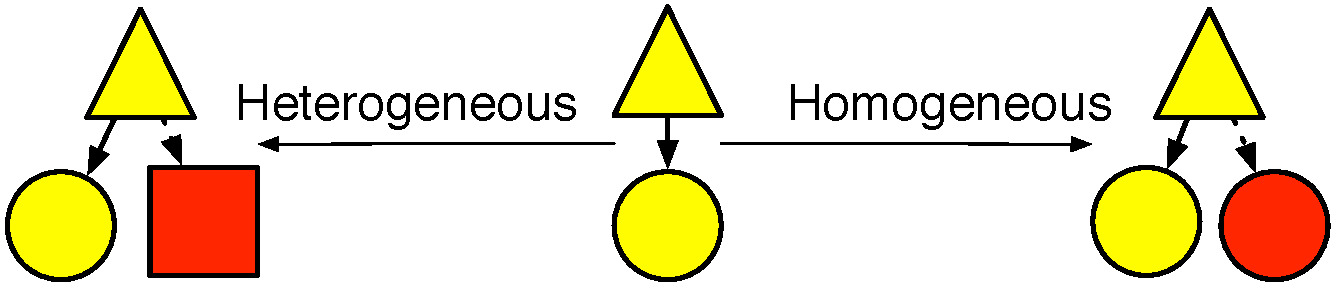
\epsfig{file=parameters/figures/HC.pdf, width=2.7in}
\caption{Appending a module.}
\label{fig:hc}
\setlength{\belowcaptionskip}{-10pt}
\end{figure}
\begin{figure}
\centering
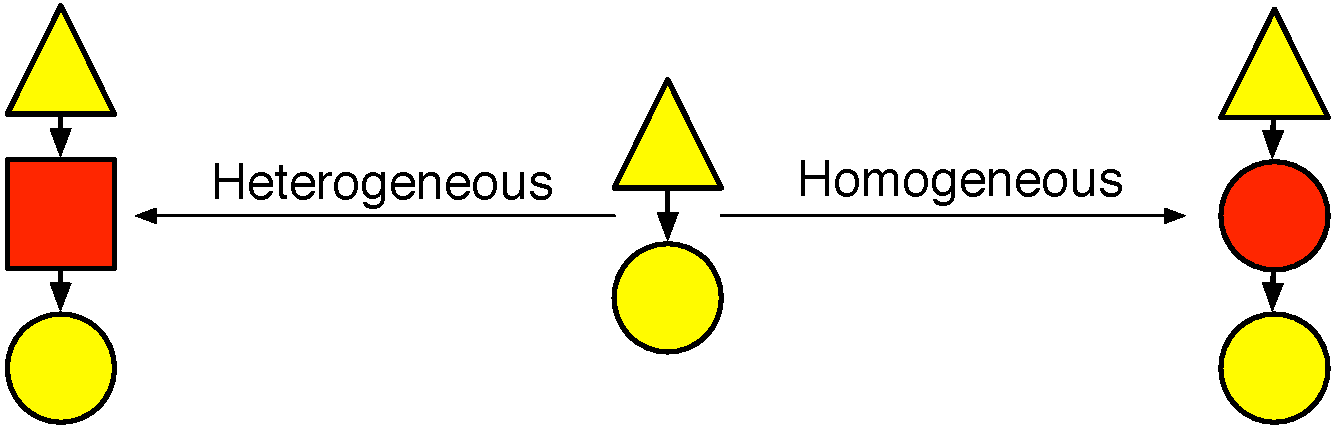
\epsfig{file=parameters/figures/VC.pdf, width=2.7in}
\caption{Inserting a module.}
\label{fig:vc}
\setlength{\belowcaptionskip}{-20pt}
\end{figure}

Within each category, the modification is either homogenous or heterogenous depending on whether the added module's type is the same as its sibling (for appending, see Figure \ref{fig:hc}) or child (for inserting, see Figure \ref{fig:vc}). In addition, we assume all added parameters require unique values assigned in the top-level list.

Each modification will trigger a varying number of parameter-related source code changes depending the existing module hierarchy, as well as the parameterization paradigm. The following attributes of a module's modification, M, are relevant to our calculation:

\begin{itemize}\itemsep1pt \parskip0pt \parsep0pt
\item $\delta$, the number of times any parent of M is instantiated
\item $\pi$, M's number of unique parent module declarations (that is not of type M)
\item $\mu$, whether M's immediate parent has M's type
\item $\theta$, the number of added parameters
\item $\rho$, the number of references to M's child's parameters from any of M's parents
\end{itemize}

Examples calculating these attributes for different module hierarchies is depicted in Figure \ref{fig:attr}.

\begin{figure}
\centering
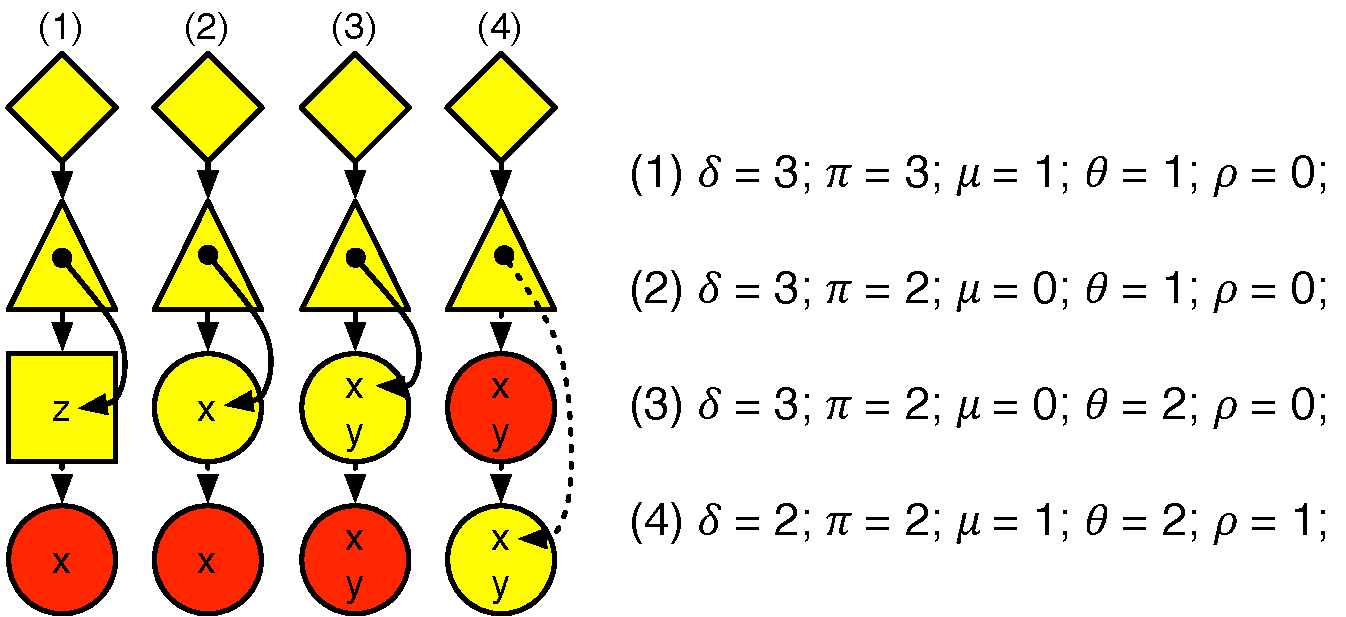
\epsfig{file=parameters/figures/CDSq.pdf, width = 3in}
\caption{(1)-(4) are example module hierarchies; module types are shapes, inserted/appended modules are red, and intermodule parameter references are curved arrows (note the broken reference in (4)).}
\label{fig:attr}
\setlength{\belowcaptionskip}{-20pt}
\end{figure}

Given these assumptions, we calculate the number of top-level, non-local, and local changes per module addition. Top-level changes are always equal to the number of parameters added ($\theta$). Local changes consist of instantiating the new module and local manipulations of the module's parameter values. Non-local changes include any other modifications, including parent instantiations, parent declarations, or modifying any parent's parameter object's instantiation/declaration. Total changes are simply the sum of all LCs, NLCs, and TLCs.

\subsection{Appends}

As shown in Table \ref{het:app} for heterogenous appends, both environment passing schemes require zero NLCs. Surprisingly, nested-struct is almost equivalent to both environment passing schemes because $\mu$ is always either 0 or 1, depending on whether the immediate parent is of the same type as the appended module.

\begin{table}
\centering
\begin{tabular*}{0.45\textwidth}{lccl}
\toprule
Paradigm    & LC & NLC & Total Changes\\
\midrule
arg-lists      &  1 & ($\delta$+$\pi$)*$\theta$ & 1+$\theta$*($\delta$+$\pi$+1)  \\
flat-struct  &  1 & $\pi$*$\theta$ &  1+$\theta$*($\pi$+1)  \\
nested-struct    &  1 & $\mu$ &  1+$\theta$+$\mu$  \\
regular-env    &  1 & 0 & 1+$\theta$ \\
cde &  1 & 0 & 1+$\theta$  \\
\bottomrule
\end{tabular*}
\caption{Appending a heterogenous module.}
\label{het:app}
\end{table}

For homogenous appends (Table \ref{hom:app}), CDEs are slightly better than nested-structs, while regular environments perform poorly with $\theta$ additional source-code changes.

\begin{table}
\centering
\begin{tabular*}{0.45\textwidth}{lccl}
\toprule
Paradigm    & LC & NLC &Total Changes\\
\midrule
arg-lists      &  1 & ($\delta$+$\pi$)*$\theta$ & 1+$\theta$*($\delta$+$\pi$+1)  \\
flat-struct  &  1 & $\pi$*$\theta$ & 1+$\theta$*($\pi$+1)  \\
nested-struct    &  1 & $\mu$ & 1+$\theta$+$\mu$  \\
regular-env    &  1+$\theta$ & 0 & 1+$\theta$*2 \\
cde &  2 & 0 & 2+$\theta$  \\
\bottomrule
\end{tabular*}
\caption{Appending a homogenous module.}
\label{hom:app}
\end{table}

\subsection{Insertions}

Table \ref{het:ins} shows that regular and CDE parameterization paradigms trigger zero NLCs, but insertions into designs using argument lists, flat-structs, or nested-structs can trigger large numbers of NLCs depending on the module's depth, number of unique parents, or number of cross-module parameter references.

\begin{table}
\centering
\begin{tabular*}{0.45\textwidth}{lccl}
\toprule
Paradigm    & LC & NLC & Total Changes\\
\midrule
arg-lists      &  1 & ($\delta$+$\pi$)*$\theta$ & 1+$\theta$*($\delta$+$\pi$+1)  \\
flat-struct  &  1 & $\pi$*$\theta$ & 1+$\theta$*($\pi$+1)  \\
nested-struct    &  1 & $\rho$+$\mu$ & 1+$\theta$+$\rho$+$\mu$  \\
regular-env    &  1 & 0&1+$\theta$ \\
cde &  1 & 0 & 1+$\theta$  \\
\bottomrule
\end{tabular*}
\caption{Inserting a heterogenous module.}
\label{het:ins}
\end{table}

Homogeneous insertions, however, clearly show that CDEs are superior to all other paradigms (Table \ref{hom:ins}). Regular environment passing is hindered by the additional $\theta$ renames, while nested-structs are limited by $\rho$, number of spanning parameter references. 

\begin{table}
\centering
\begin{tabular*}{0.45\textwidth}{lccl}
\toprule
Paradigm    & LC & NLC & Total Changes\\
\midrule
arg-lists      &  1 & ($\delta$+$\pi$)*$\theta$& 1+$\theta$*($\delta$+$\pi$+1)  \\
flat-struct  &  1 & $\pi$*$\theta$ & 1+$\theta$*($\pi$+1)  \\
nested-struct    &  1 & $\rho$+$\mu$ & 1+$\theta$+$\rho$+$\mu$  \\
regular-env    &  1+$\theta$ & 0 & 1+$\theta$*2 \\
cde &  2 & 0 & 2+$\theta$  \\
\bottomrule
\end{tabular*}
\caption{Inserting a homogenous module.}
\label{hom:ins}
\end{table}

The single LC to CDEs is from modifying the parameter object's context prior to passing it to the inserted module, which is necessary to avoid the namespace renaming of regular environment passing.

\subsection{Summary of Analysis}

Small designs with a shallow module hierarchy (e.g. a multiplier) are manageable with argument lists because the number of modification is limited. Any other design should move to a different paradigm.

Designs with shallow but wide hierarchies have few cross-module parameter references (e.g. networks) - insertions are rare and these designs are robust with nested-struct paradigms.

Deep hierarchical designs with minimal module reuse have heterogeneous insertions/appends and few parameter namespace collisions (e.g. a processor). These designs will remain robust with regular environment passing.

Complicated designs with deep hierarchies, significant module reuse, and many cross-module references have hetero- and homogeneous appends/insertions (e.g. SoC generator); these designs clearly benefit from CDEs.

\section{Implementation}
\label{sec:dse}

We augmented Chisel by leveraging its host language, Scala, to enable any Chisel design to use CDEs. At a high level, CDE values are not constant; they are functions whose arguments are (1) the query (\code{pname}) and (2) the CDE originally queried (\code{site}). The original CDE queried implicitly passes itself with every query. Ignoring the \code{site} argument turns the CDE into a regular environment; fancier parameter values based on querying \code{site} of existing parameters are now possible. For more detail, see the open-source implementation and documentation (\url{https://github.com/ucb-bar/chisel}).

%Though formulaic environment variables are nice, our motivating reason for implementing CDEs w.r.t. hardware generation was allowing the top-level parameter assignment to see "geographic" information about the component executing the query so that it may dispatch to different values accordingly. This requires that components in a library built around CDEs follow the practice of placing geographic information as new parameters in the environments they produce for their children at the point where such geographic distinctions are clear. For instance, a "network" component will instantiate and wire together many child "node" components. We would like a convenient way to assign different parameter values to the nodes based on their location in the topology. To achieve this we place the burden on the parent (network) to annotate each node's inherited CDE with a constant parameter like [location = \$ -> (x,y)] so the top-level environment can tune each node's behavior according to location by referencing it in the function [foo = \$ -> ...expression dependent on \$location...].

\section{Conclusion}
\label{sec:con}

We have presented a taxonomy of existing parameterization paradigms in HDLs and demonstrated that our context-dependent environments paradigm is provably more robust in the face of modification to any given design's module hierarchy. Our implementation of CDEs within Chisel allowed us to perform a design space exploration composing multiple hardware generators, solely by changing the top-level environment.

%There is little benefit to using a context-dependent environment over a normal environment when most modifications to a design are only heterogenous. Unfortunately, more complicated designs often have homogeneous structures and, in this case, context-dependent environments are significantly superior. Use CHISEL because we've implemented context-dependent environments!!
